\section*{Exercice 189 -- Géométrie -- Vérins}
\setcounter{exo}{0}
%CCMP PSI 2009 Roburoc

\begin{obj}
Déterminer la course des vérins en fonction de l’amplitude du mouvement ainsi que la pression maximale $p_{\text{maxi}}$ dans le circuit hydraulique.
\end{obj}

Le modèle cinématique retenu est défini sur la figure suivante.


\begin{center}
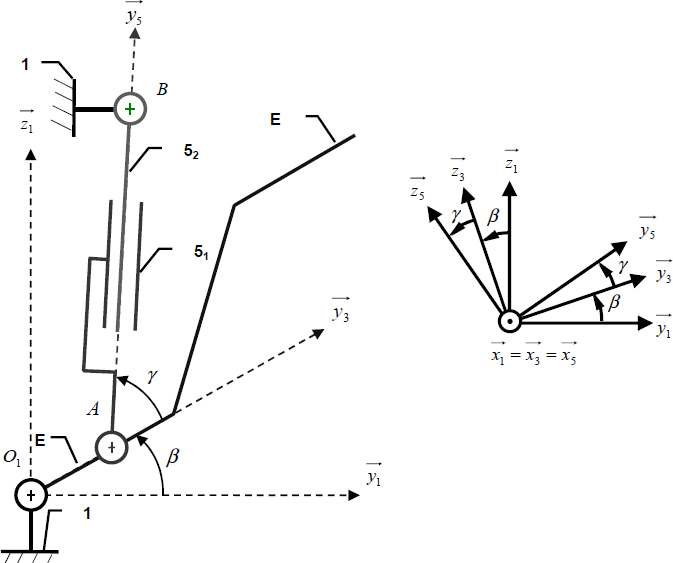
\includegraphics[width=\linewidth]{993_01}
\end{center}

Le mécanisme est constitué :
\begin{itemize}
\item du pode central fixe 1 : repère associé $\rep{1}=\repere{O_1}{x_1}{y_1}{z_1}$
\item de l’ensemble E=\{bras d’articulation avant \textbf{4} + pode avant \textbf{3} + roues avant\} : repère associé 
$\rep{3}=\repere{O_1}{x_1}{y_3}{z_3}$ avec $\beta=\angl{y_1}{y_3}=\angl{z_1}{z_3}$;
\item du vérin 5 constitué du corps $5_1$ et de la tige $5_2$ : repère associé $\rep{5}=\repere{A}{x_1}{y_5}{z_5}$ 
 avec $\gamma=\angl{y_3}{y_5}=\angl{z_3}{z_5}$;
\item du vérin 6 non représenté car ayant le même comportement que le vérin 5.
\end{itemize}

Paramétrage : $\vect{O_1A}=d_4\vect{y_3}$; $\vect{AB}=\lambda\vect{y_5}$; $\vect{O_1B}=d_1\vect{y_1}+h_1\vect{z_1}$.

Valeurs numériques : $d_4 = \SI{70}{mm}$; $h_1 = \SI{292}{mm}$; $d_1 = \SI{76}{mm}$; $\beta\in\left[-45\degres;+30\degres\right]$.



\subparagraph{}
\textit{Exprimer $\lambda$ en fonction de $d_1$, $h_1$, $d_4$ et $\beta$.}
\ifprof
\begin{corrige}
\end{corrige}
\else
\fi


\subparagraph{}
\textit{Calculer les valeurs numériques d’élongation minimale $\lambda_{\text{min}}$ , maximale $\lambda_{\text{max}}$ ainsi que la course du vérin 5.}
\ifprof
\begin{corrige}
\end{corrige}
\else
\fi


L’objectif suivant est d’évaluer les pressions maximales s’exerçant dans le circuit hydraulique dans la configuration
d’essai décrite précédemment à savoir :
\begin{itemize}
\item le pode central 1 est fixe et placé parallèlement au sol ;
\item  les podes avant 3 et arrière 2 ne sont pas en contact avec le sol et un angle de tangage est alors imposé aux
podes avant et arrière par rapport au pode central.
\end{itemize}
Sur la figure suivante, l’évolution du rapport entre les efforts exercés par les vérins avant 5 et 6 et le poids de l’ensemble E a
été tracée en fonction de l’angle de tangage $\beta$. La masse de l’ensemble E est $m_E=\SI{60}{kg}$.

\begin{center}
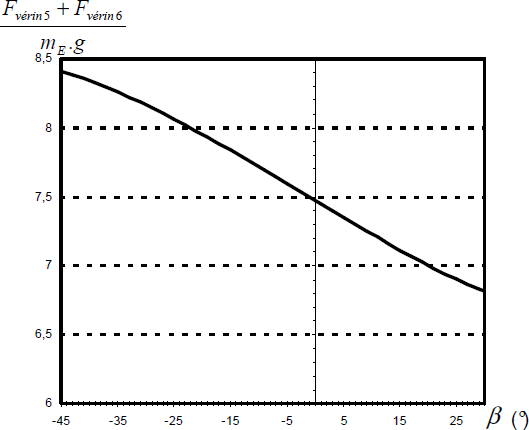
\includegraphics[width=\linewidth]{993_02}
\end{center}

\subparagraph{}
\textit{À partir du tracé précédent et du plan du vérin, déterminer la valeur de la différence de
pression maximale $\Delta P _{\text{max}}$ entre les deux chambres des vérins avant 5 et 6.}
\ifprof
\begin{corrige}
\end{corrige}
\else
\fi


\begin{center}
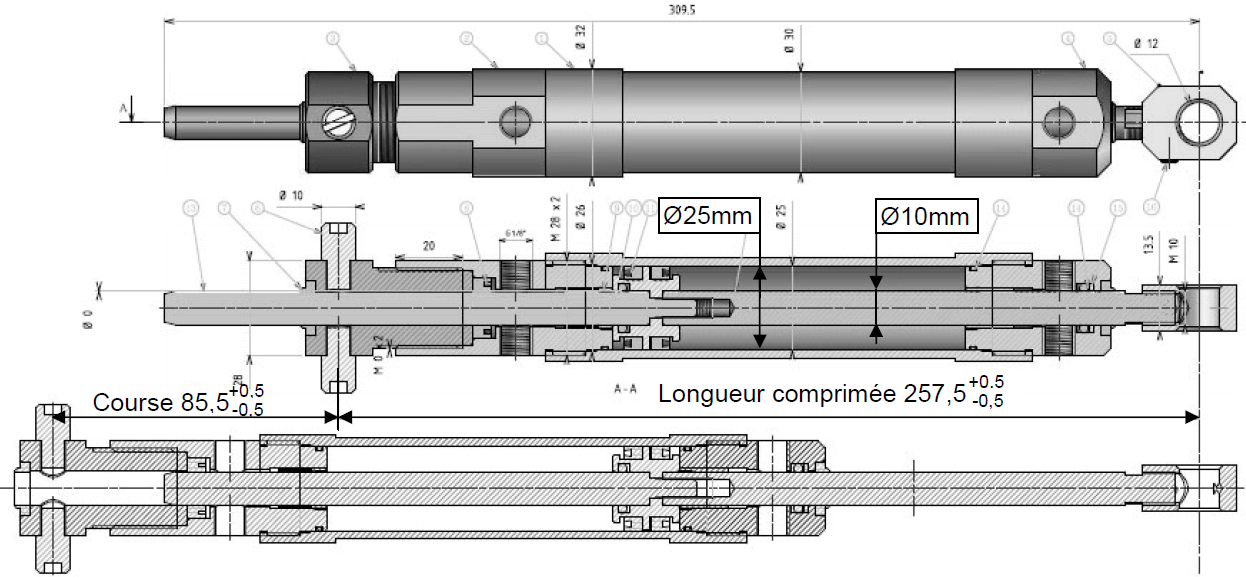
\includegraphics[width=\linewidth]{993_03}
\end{center}

La pression minimale dans le circuit hydraulique est supposée constante et égale à $p_0$ ($p_0 = \SI{1}{bar}$)). Des limiteurs de pression tarés à \SI{150}{bars} sont placés en sortie du distributeur 4/3.

\subparagraph{}
\textit{Déterminer l’expression de la pression maximale  $p_{\text{maxi}}$ dans le circuit hydraulique en fonction de $p_0$ et $\Delta P _{\text{max}}$. Réaliser l’application numérique.}% et comparer cette valeur à la pression de tarage des limiteurs.}
\ifprof
\begin{corrige}
\end{corrige}
\else
\fi
